\chapter{Problemfelder innerhalb des Change Managements}
\label{problemfields}

% - erster Hauptteil der Arbeit
% - Herausarbeitung von Veränderungsprozessen und Problemfelder innerhalb der DT

Nach den theoretischen Ausführungen der vorangestellten Kapiteln soll nun inhaltlich auf den ersten Hauptschwerpunkt der vorliegenden Arbeit eingeführt werden. Um in \ref{agilepractices} eine Reihe agiler Methoden hinsichtlich ihrer Anwendbarkeit in Problemfeldern der Digitalen Transformation zu evaluieren, müssen letztere zunächst erarbeitet werden. Dafür soll ein systematisches Literaturreview (\gls{SLR}) vorgenommen werden. Aus diesem werden  zunächst Veränderungsprozessmuster innerhalb des Transformationsprozesses  zusammengefasst.  Zusätzlich werden auf  Grundlage dessen eine Reihe von problematischen Schwerpunkten erarbeitet. Nachfolgend soll zunächst das methodische Vorgehen im aktuellen Kapitel geschildert werden. Es schließt sich eine gesonderte Übersicht der erschlossenen Literatur an, auf dessen Grundlage  die Ergebnisse aufgeführt werden.  

\section{Methodisches Vorgehen}
\label{problemfields:methods}

% - genaue Darstellung über Vorgehen in der SLR + Metastudie
% - Suchmethodik, Keywords, Kriterien, Auswahlprozes ...
% - https://docs.google.com/document/d/1wzYRearLcVTlKJxPp6Mz5U860VoXzkNX7armGeCoxt4/edit

Nachfolgend soll das genaue methodische Vorgehen des ersten systematischen Literaturreviews vorgestellt werden. Vor der eigentlichen Suche nach Fallstudien bzw. relevanter Literatur zum Thema der Digitalen Transformation, wurde eine einheitliche Suchstrategie aufgestellt. Diese wird in \ref{fig:suchstrategie} dargestellt. 

\begin{figure}[H]
	\centering
	\fbox{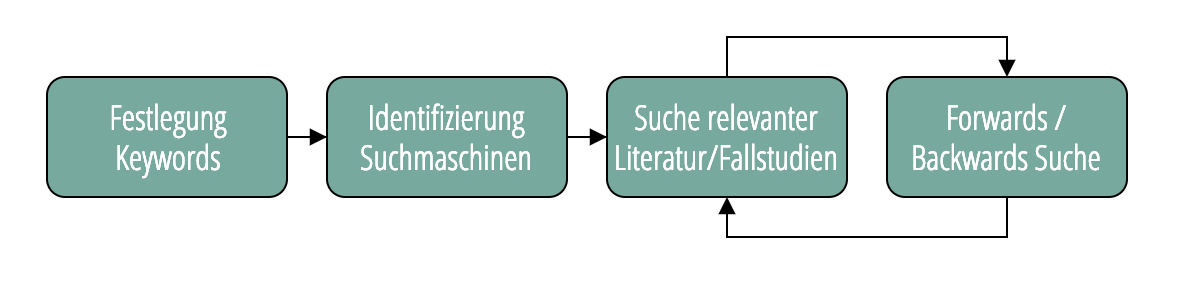
\includegraphics[width=0.8\linewidth]{pics/suchstrategie}}
	\caption[Suchstrategie des SLR]{Suchstrategie des SLR (eigene Darstellung)}
	\label{fig:suchstrategie}
\end{figure}

Wie der Abbildung zu entnehmen wurden zunächst \textit{Keywords} für die  Literatursuche festgelegt. Diese wurden nach einer ersten Probesuche zunehmend angepasst, bis eine zufriedenstellende Ergebnismaske erzielt wurde. Da in der Suche englische  und deutsche Literatur eingeschlossen wurde, wird im folgenden zwischen englischen und deutschen Keywords unterschieden. In \ref{tab:keywordsslr1} werden nachfolgend die \textit{Keyword-Suchketten} aufgeführt, die in sämtlich genutzten Literatursuchmaschinen verwendet wurden. Die Syntax der Suchketten kann dabei  von Suchmaschine zu  Suchmaschine variieren, die Übersicht dient der Allgemeinheit.

\begin{table}[ht]
	\centering
	\caption{Übersicht Keyword-Suchketten SLR 1}
	\begin{tabular}{|p{7cm}|p{7cm}|}
		\hline
		\textbf{Deutsche Keywords}& \textbf{Englische Keywords} \\
		\hline
		digitale+transformation+fallstudie OR digitalisierung+fallstudie   & digital+transformation+case OR digitalization+case \\
		\hline
	\end{tabular}
	\label{tab:keywordsslr1}
\end{table}

Weiter wurden im Vorfeld relevante Literatursuchmaschinen identifiziert. Dabei wurde darauf geachtet, dass überwiegend Suchmaschinen mit Zugang zur technischer sowie wirtschaftlicher Relevant gewählt wurden. Grundsätzlich wurden überwiegend Datenbanken mit vorhandenem Online-Zugang genutzt. \todo{weiter ausführen?} \ref{tab:suchmaschinenslr1} zeigt hierbei  eine Übersicht der genutzten Suchmaschinen mit Angabe der insgesamt gefundenen Literatur.

\begin{table}[ht]
	\centering
	\caption{Übersicht Literatursuchmaschinen SLR 1}
	\begin{tabular}{|p{5cm}|p{7cm}||p{3cm}|}
		\hline
		\textbf{Datenbank/Bibliothek}& \textbf{URL} &  \textbf{Treffer Keywords  (summiert)} \\
		\hline
		IEEE Xplore & \url{https://ieeexplore.ieee.org} & 770 \\
		(Online) - Bibliothek Hochschule Harz & \url{https://opac.lbs-magdeburg.gbv.de/DB=4/LNG=DU} & 6 \\
		(Online) - Bibliothek Technische Universität Berlin  & \url{https://www.ub.tu-berlin.de/literatur-suchen}& 1 \\
		Google Scholar &  \url{https://scholar.google.de}  & 26.800 \\
		Scopus & \url{https://www.scopus.com} & 4.347 \\
		ResearchGate & \url{https://www.researchgate.net} &Keine Angabe vorhanden \footnotemark \\ 
		ACM Digital Library & \url{https://dl.acm.org} & 174.857 \\
		\hline
	\end{tabular}
	\label{tab:suchmaschinenslr1}
\end{table}

\footnotetext{\textit{ResearchGate} bietet keine Funktion zur Angabe der kompletten Treffer-Zahl}

Die Angaben zu den Literatur-Treffern in den einzelnen Suchmaschinen zeigt klar, dass eine weitere Filterung vorgenommen werden musste. Dafür wurden ein \textit{Auswahlprozess} definiert, um nur relevante Fallstudien für die folgenden Untersuchungen zu inkludieren.

\todo{Auswahlprozess}
\todo{Ein - und  Ausschlusskriterien}
\todo{Übersicht Zahlen gefundene Literatur}
\todots

\section{Literaturübersicht}

% - Fallstudien
% - tabellarische Darstellung (https://docs.google.com/document/d/1caHZ-pLGa\_L-TfO4nOh2zZLdAa5nazKaoUZDeDmN90M/edit)
% - Inhaltsangabe jeder Arbeit (Zusammenfassung)

\todo{Siehe Tabelle A1 und A2 im Anhang}

\todots

\section{Veränderungsprozessmuster innerhalb der Digitalen Transformation}
\label{problemfields:changepatterns}

% - tabellarische Kreuzmatrix (siehe Link oben)
\todo{Siehe Tabelle A3 im Anhang}

\begin{table}[ht]
	\centering
	\caption{Auswertung Clustering Veränderungsprozessmuster (kurz)}
	\begin{tabular}{|c|c|}
		\hline
		\textbf{Veränderungsprozessmuster}& \textbf{Anzahl Nennungen} \\
		\hline
		Einführung einer Multi-Kanal-Strategie   & 6  \\
		Wechsel vom Offline- zum Online-Vertrieb & 5  \\
		Erschaffung neuer digitaler Produkte     & 12 \\
		Tendenz zur Kundenorientierung           & 16 \\
		Digitalisierung des Geschäftsmodell      & 11 \\
		Digitaler Wissensaufbau im Unternehmen   & 12 \\
		Datengestützte Verbesserungsprozesse     & 5  \\
		Erzeugung eines digitalen Ökosystems     & 7  \\
		Digitalisierung von internen Prozessen   & 7  \\
		Einbindung innovativer Technologien      & 6  \\
		Aufbau technisches Sicherheitskonzept    & 4  \\
		Digitale Neuausrichtung der Organisation & 13 \\
		Innovationsförderung                     & 7  \\
		Kooperation mit externen Treibern        & 5 \\
		\hline
	\end{tabular}
	\label{tab:clusteringvpshort}
\end{table}

\todots

\section{Identifikation von Problemfeldern}

% - tabellarische Kreuzmatrix (siehe Link oben)
\todo{Siehe Tabelle A4 im Anhang}

\begin{table}[ht]
	\centering
	\caption{Auswertung Clustering Problemfelder (kurz)}
	\begin{tabular}{|c|c|}
		\hline
		\textbf{Problemfeld}& \textbf{Anzahl Nennungen} \\
		\hline
		Unternehmensweite Kommunikationsprobleme        & 5  \\
		Festhalten an verfestigten Strukturen           & 7  \\
		Zeit - und Marktdruck                           & 5  \\
		Unterschätzung der Komplexität                  & 4  \\
		Fehlende Kontinuierliche Verbesserungsprozesse  & 7  \\
		Störung durch oberes Management (Top-Down)      & 7  \\
		Konflikte zwischen IT und Business              & 4  \\
		Fehlende frühe Einbeziehung aller Mitarbeiter   & 3  \\
		Sicherheitsprobleme                             & 2  \\
		Fehlende Kundenorientierung                     & 13 \\
		Fehlendes technischen Know-How                  & 10 \\
		Fehlende monetäre Ressourcen                    & 2  \\
		Rechtliche Bestimmungen und Datenschutz         & 5  \\
		Fehlende Transparenz (intern und extern)        & 4  \\
		Fehlende Partnerschaften                        & 6  \\
		Fehlende Innovationskultur                      & 6  \\
		Langsame Entscheidungsprozesse                  & 3  \\
		Unternehmenskulturelle Probleme                 & 8  \\
		Fehlendes Vertrauen, Akzeptanz und Bereitschaft & 9  \\
		Unklare Verantwortlichkeiten                    & 5  \\
		Fehlende digitale Strategie                     & 6 \\
		\hline
	\end{tabular}
	\label{tab:clusteringpfshort}
\end{table}

\todots

\section{Zusammenfassung}


